\section{Codierung}
% Was ist eine Codierung
Unter der Codierung eines Individuums versteht man eine Informationskette, die die relevanten Erbinformationen enthält.
% Codierung in der Natur
Die Gene eines Menschen können so als dessen Codierung angesehen werden.
% Codierung bei den Evolutionsstrategien
Bei den Evolutionsstrategien wurde auf eine komplizierte Codierung verzichtet und dafür eine sehr kurze Codierungsform eingesetzt \cite[S.147]{schoeneburg}. Die relevanten Erbinformationen von Individuen werden durch Vektoren reeller Zahlen dargestellt \cite[S.147]{schoeneburg}. Diese Vektoren werden Chromosome genannt. Jedes Individuum hat ein solches Chromosom.
Eine Menge an Individuen bildet eine Population. Diese Codierungsweise wird in der Grafik \ref{fig:codierung} dargestellt. Darin ist zu sehen, wie eine Menge an Individuen eine Population bildet. Die Individuen sind als Männchen verbildlicht. Darüber hinaus ist ein Chromosomausschnitt zu sehen.\\
Die Wahl für diese Codierungsvariante lässt sich darauf zurückführen, dass die Evolutionsstrategien zu Beginn für ingenieurstechnische Optimierungen verwendet wurden \cite[S.147]{schoeneburg}.
In diesem Aufgabenfeld werden optimale Systemparameter gesucht. Diese lassen sich sehr gut als Vektoren reeller Zahlen abbilden.\\
Der durch die Evolutionsstrategien gewählte Codierungsansatz wird als phänotypisch orientiert bezeichnet \cite[S.148]{schoeneburg}. Das bedeutet, dass im Gegensatz zu einer genotypischen Orientierung, die Eigenschaft des Individuums betrachtet wird, die sich aus den Chromosomen ergeben, und nicht die Chromosome selbst.
Die Eigenschaft des Individuums kann durch Qualitätsfunktionen berechnet werden.

\begin{figure}[!htb]
	\centering
	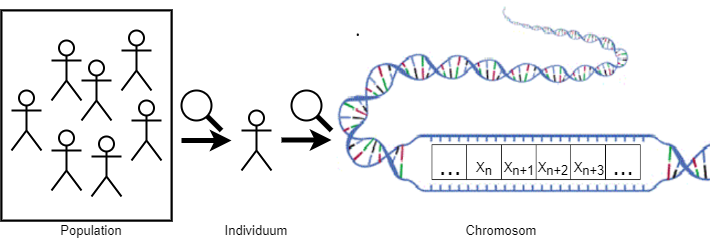
\includegraphics[width=1.\textwidth]{img/codierung/codierung.png}
	\caption{Grafische Darstellung einer Population, von Individuen und eines Chromosoms.}
\label{fig:codierung}
\end{figure}


